\begin{figure}[ht]
    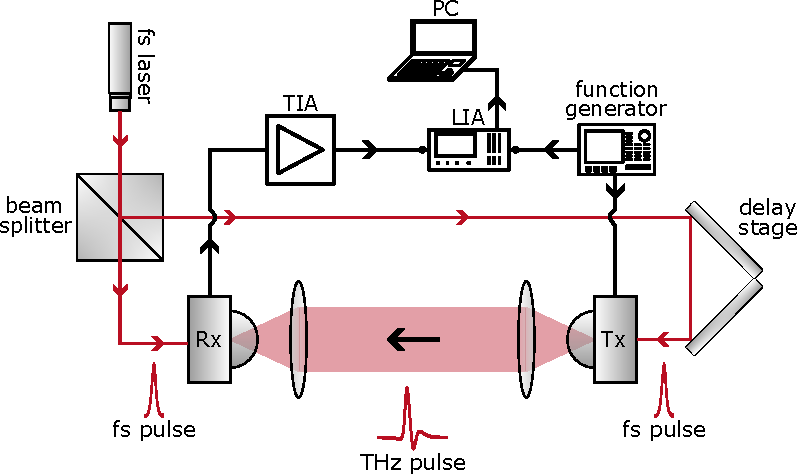
\includegraphics[width=0.9\linewidth]{figures/TDS_schematic.pdf}
    \centering
    \caption{Schematic diagram of the setup used for THz-TDS.}
    \label{fig_TDS}
\end{figure}

Generation and detection of THz radiation in a pulsed system were described in detail in Section \ref{sec_gen_det}. Only a brief overview will be given here. The TSD setup (see Figure \ref{fig_TDS}) used for characterization of the fabricated H-Dipole antennas utilizes a modified MenloSystems C-Fiber \cite{FemtosecondErbiumLaser} laser system with a pulse duration of \num{90} \si{\femto \s}, a repetition rate of \num{100} \si{\mega \hertz} and an optical wavelength of \num{1560} \si{\nano \meter}. The laser signal is coupled out using glass fibers. In order to achieve coherent signal detection, the THz-TDS setup utilizes a closed-loop system. Both the pump beam and the probe beam necessary for THz generation and detection with PCAs are generated using the same laser beam. The fibers drive both the detector and the emitter with \num{25} \si{\milli \watt} of power each. The THz signal is generated with the help of the pump beam and ultimately detected by sampling the temporal overlap of the probe beam and the THz field. This closed-loop approach ensures that the THz-TDS system provides high SNR and DNR. A beam splitter is utilized to split the initial laser pulse into the two needed signals. 

On the transmission side of the setup, one of the two laser signals passes through a delay stage before being fed into the transmitter (Tx) developed in \cite{nandiErAsInAlGaAsPhotoconductors2021}. The transmitter primarily consists of a PCA mounted on a hyper-hemispherical silicon lens with a radius of \num{6.1} \si{\milli \meter}. The device is fully packaged, featuring an APC-fiber for the laser signal and a SMA connector for applying the bias voltage. The package has a cylindrical shape with a length of \num{5} \si{\centi \meter} and an outer diameter of \num{6} \si{\centi \meter}. Additionally, the packaging includes a fiber collimator and a focusing lens to ensure efficient coupling of the laser signal into the device. The PCA is DC-biased until a current of approximately $180$ \si{\micro \ampere} is reached, enabling the acceleration of free charge carriers generated by the laser signal. This typically corresponds to a bias voltage of around \num{180} \si{\volt}. The fully packaged transmitter is mounted on a one-dimensional stage to horizontally align the THz field. When illuminated by the laser signal, the PCA emits THz radiation. The THz field travels through free space and is focused onto the receiving port by two lenses.  

As demonstrated in Section \ref{sec_gen_det}, the signal at the receiver in this setup can be approximated as the convolution of the delta-function and the incident THz transient. Hence, a mechanical delay stage is needed before the laser signal reaches the transmitter to scan through the complete THz pulse. By varying the relative delay between the THz signal and the optical probing pulse, the complete THz pulse received by the antenna can be extracted. 

The second laser signal is directly coupled to the receiving port (Rx) of the setup. The receiver consists of an antenna that is being used to work as a recipient for THz radiation.  In this thesis, the receiving port of the setup is an antenna of the fabricated probe, which serves as the device under test (DUT). The DUT is mounted on a hyper-hemispherical silicon lens with a radius of \num{6.1} \si{\milli \meter}, using vacuum grease for attachment. A fiber collimator and a focusing lens are employed to direct the laser pulse onto the active region of the DUT. Two three-dimensional stages are used: one for aligning the laser signal with the DUT, and another for aligning the DUT with the incident THz transient.

For a PCA to work as a receiver, the device is illuminated by the femtosecond laser pulse, the probing pulse. By illuminating the device, free electron-hole pairs are generated. The incoming THz radiation, which is to be measured by the receiving port, biases the device. The illumination and biasing of the device results in a DC photocurrent. This current is proportional to the convolution of the incoming THz transient and the optical probing signal. The DC current can be read out using probing needles at the antenna pads and post detection electronics. As the measured photocurrent is generally very small (around $10^{-9} ... 10^{-6}$ \si{\ampere}), the signal is transformed to a voltage and amplified by a trans-impedance amplifier (TIA) from TEM-Messtechnik (PDA-S) \cite{PDASPhotodiodenVerstaerker}. With the TIA, gains of up to $\sim 10^7 $ \si{\volt}/\si{\ampere} can be achieved. The THz signal needs to be extracted from background noise. A Lock-In Amplifier (LIA) is used for signal extraction. The input signal is multiplied with a reference signal (demodulation), which is usually a sine-wave, and then filters the result using a low-pass filter. This isolates the desired signal at a specific frequency from noise and other frequency components. The frequency at which the demodulation takes place is the same frequency used for modulating the THz transmitter. A LIA from Zurich Instruments (MFLI-MD) \cite{MFLI500KHz2019} is employed for demodulation of the incoming signal. A graphical user interface provided by MenloSystems is used for data acquisition and storage. For all measurements, a scanning window of \num{100} \si{\pico \s} is employed. The data is recorded with an integration time of \num{1000} \si{\s} to achieve the highest possible SNR. The time-domain data is saved for further data analysis.